\section{Durchführung}
\label{sec:Durchführung}

%2.1
\subsection{Messreihe zur Bestimmung der Zeitkonstanten im RC-Kreis anhand des Entladevorgangs}

Zunächst wird zur Bestimmung der Zeitkonstante ein Spannungsgenerator
wie in Abbildung \ref{fig:v353_1} dargestellt an das RC-Glied angeschlossen und eine Rechteckspannung angelegt.
Mithilfe eines digitalen Oszilloskops und der Trigger-Funktion wird die abfallende 
Flanke dargestellt. Die Spannung am Kondensator wird in Abhängigkeit der Zeit gemessen, und es werden mindestens 10 Werte notiert.
Dass die Entladung beginnt erkennt man daran, dass die Spannung von ihrem Maximalwert auf Null zurück springt.
\begin{figure}[H]
  \centering
  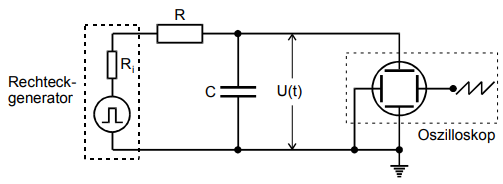
\includegraphics{V353_1.png}
  \caption{Messschaltung zur Bestimmung der Zeitkonstanten mittels Beobachtung des 
  Entladevorgangs. \cite[S. 6]{kent}}
  \label{fig:v353_1}
\end{figure}

%2.2
\subsection{Messreihe zur Bestimmung der Spannungsamplitude des Kondensators
im RC-Kreis}
Als nächstes wird eine Sinusspannung $U_\text{0}(t)$ angelegt und die 
Amplitude $A$ der Kondensatorspannung $U_\text{C}(t)$ in Abhängikeit der Frequenz gemessen.
Es werden 30 Frequenzen $\omega$ im Bereich von 100 bis 10000
$\si{\hertz}$ eingestellt und mit der Cursor-Funktion die dazugehörige Kondensatorspannung 
$U_\text{C}(t)$ gemessen. Dabei werden für jede Zehnerpotenz je 10 Werte gemessen.

%2.3
\subsection{Messreihe zur Bestimmung der Phasenverschiebung im RC-Kreis}
In der dritten Messreihe wird die Phasenverschiebung $\phi$ zwischen der generierten 
Spannung $U_\text{G}(t)$ und der Kondensatorspannung $U_\text{C}(t)$ bestimmt.
Hierzu wird die Schaltung so verändert, dass die generierte Spannung ebenfalls auf 
dem Oszilloskopen dargestellt werden kann (Abbildung \ref{fig:v353_3}) und die Signale 
werden übereinander 
symmetrisch zur $t$-Achse ausgelegt. Mithilfe der Cursor-Funktion wird dazu der Abstand
$a$ zwischen den zugehörigen Nulldurchläufen gemessen (Abbildung \ref{fig:phi}), wobei
die Periodendauer $b$ durch die Frequenz $\omega$ gegeben ist. Die eingestellte Frequenz
ist dabei die gleiche wie im vorherigen Durchführungsteil, es werden also wieder 30 Frequenzen eingestellt.
\begin{figure}[H]
  \centering
  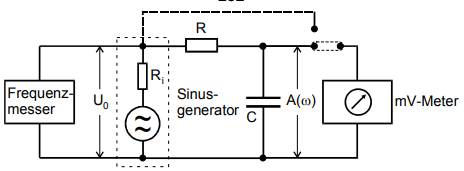
\includegraphics{V353_2.png}
  \caption{Messschaltung zur Bestimmung der Phasenverschiebung $\phi$. \cite[S. 7]{kent}}
  \label{fig:v353_3}
\end{figure}
\begin{figure}
  \centering
  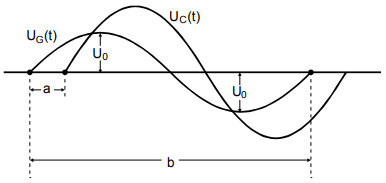
\includegraphics{phi.png}
  \caption{Messung der Phasenverschiebung zwischen zwei Spannungen mit dem
Zweistrahloszilloskopen. \cite[S. 7]{kent}}
  \label{fig:phi}
\end{figure}

%2.4
\subsection{Messreihe zur Bestätigung der Integratorfunktion des RC-Kreises}
Um die Integratorfunktion des RC-Kreises zu überprüfen, wird eine ausreichend hohe
Frequenz $\omega$ eingestellt und eine Rechteckspannung angelegt. Das Oszilloskop 
zeigt sowohl die angelegte als auch die integrierte Spannung an. Als zweites wird eine
Dreieckspannung angelegt. Die letzte Einstellung ist eine Sinusspannung. Die Ergebnisse
werden als Bilder gespeichert.